% ------------------------------------------------------------------------
% A Latex "template" for CMP MSc Dissertation. 
% 
%
% Please read the brief Instructions (Instrucrtions.tex) below and in sample files 
% to learn how to use this option in this template.
%
%
% Notes and sample files:
% "acronymNotes.tex": brief introduction on how to make a LOA. 
% "acronyms.tex": a sample file where you define abbreviations.
%  
%   
% Brief Instructions
%#### 
%% Preparations: 
% (i)  Download the zipped Latex templat file into your disk or your university's home space on U disk,
% (ii) Unzip all the fiels into your working folder, such as \Dissertation. 
% (ii) Change/replace/fill few places in this "DissertationTemplate.tex" file to suit your need:
% 		such as, Your course, Year, Dissertation title, your name, markers, etc.
%
%% Then you can follow teh following instructions(not necessarily in that order) to write your dissertation. 
%   
%% 1. Write your abstract in a separate tex file and name it as ABS.tex
%% 2. Write your acknowledgement in a separate tex file and name it as ACK.tex  
%    Note: Both ABS.tex and ACK.tex files are already included in the style file. 
%
%% 3. wirte each chapter in a separate tex file and name e.g. Ch1, Ch2, etc. 
% and then use "include" to inlcude them as shown in this example.
% 
%#### 
% If you wish to produce a list of abbreviations/acronyms 
% that are used in your dissertation, you must read notes 4-7 below. 
%
%% 4. Define abbreviations or acronyms
% 	you can use the given sample file "acronyms.tex" 
% 	to define your abbreviations or acronyms, and 
% 	some examples are already defined in that file.
% 	After you have defined them, (you can add any new items anytime you like), 
% 	save it in the same folder as this "DissertationSample1.tex"
% 	as it is included by using "include{acronyms}" in this file later.
% 	Note: if you use any other file name, change it in "\inlcude{yourFilename}. 
%
%% 5. Using the defined abbreviations/acrynoms
%   In file "acronymNotes.tex", I give some notes and few examples 
%   to explain and show how to use defined acrynoms in your tex file.  
%
%% 6. Generate a List of Abbreviations(LOA)
%  You must issue command "Makeglossaries" to produce few more auxiliary files 
%   e.g. xxxx.acr, and/or .glo, and/or .gls, etc. in order to produce LOA 
%   so, is you use TexStudio, Click "Tools" and choose "Makeglossaries"
%
%% 7. Don't want to have a list of Abbreviations
%  use command "\nolistofabbs", by uncomment it in later part  
%  then LOA will not be generated and not appear in the TOC. 
%  note: you may have to run "Build and View" twice to get the intended result.
%        first run to remove/get the acutal list of abbreviation
%		 second run to remove/get the list appearing on TOC.   
% 
%% 8. Using footnote. (% wjw, added this note on 11/09/2015)
%	If you want to use footnotes in any chapters of your dissertation, 
%	you can use command \footnote{your footnote text} in where you want.
% 	The footnotes are numbered automatically and continuously within a CHAPTER.   
%   
%% 9. Citation styles:
%   Add package "natbib" onto the preamble of your dissertation file 
%   if it is not added, using "\usepackage{natbib}"
%   (i) Use Command "\citep{...}" to produce the styyle: (Authors, year)
%   (ii) Use Command "\citet{...}" to produce the style: Authers (year)
%
%
% Disclaimer: This template is provided as it is. 
% You are welcome to try it, 
% but Dr. Wang won't be held responsible for any problems it has or causes.
% 
%
% ------------------------------------------------------------------------
\documentclass[a4paper, 12pt]{report}
\usepackage[centertags]{amsmath}
\usepackage{amsfonts}
\usepackage{amssymb}
\usepackage{amsthm}
\usepackage{newlfont}
\usepackage{graphicx}
\usepackage{natbib} % by wjw 22/11/2016 to replace apalike package
%\usepackage{pdfsync} %PDF Forward Search

\usepackage[acronym]{glossaries} % added by wjw on 05/08/15
%\usepackage{datetime}

\usepackage{CMPDissertation3a} % CMP Dissertation Style

\usepackage{XTocinc} % Include Table of Contents as the first entry in TOC

\usepackage{setspace}  % added by wj on 11/09/15
% Note: this makes the body text in chapters are double spaced 
% and text in table are single spaced.
% If you want to have a double space in tables, commented it out. 


%\usepackage[active]{srcltx}  %SRC Specials for DVI search

% Fuzz -------------------------------------------------------------------
\hfuzz2pt % Don't bother to report over-full boxes if over-edge is < 2pt
% Line spacing -----------------------------------------------------------
\newlength{\defbaselineskip}
\setlength{\defbaselineskip}{\baselineskip}
\newcommand{\setlinespacing}[1]%
           {\setlength{\baselineskip}{#1 \defbaselineskip}}
% As the package setspace is included above, which define linespacing, 
% the following newcommands for double/single spacing become redeundant, 
% hence they were commentted out. wj 11/09/2015   
%\newcommand{\doublespacing}{\setlength{\baselineskip}{2.0 \defbaselineskip}}
%\newcommand{\singlespacing}{\setlength{\baselineskip}{\defbaselineskip}}

% MATH -------------------------------------------------------------------
\newcommand{\A}{{\cal A}}
\newcommand{\h}{{\cal H}}
\newcommand{\s}{{\cal S}}
\newcommand{\W}{{\cal W}}
\newcommand{\BH}{\mathbf B(\cal H)}
\newcommand{\KH}{\cal  K(\cal H)}
\newcommand{\Real}{\mathbb R}
\newcommand{\Complex}{\mathbb C}
\newcommand{\Field}{\mathbb F}
\newcommand{\RPlus}{[0,\infty)}
%
\newcommand{\norm}[1]{\left\Vert#1\right\Vert}
\newcommand{\essnorm}[1]{\norm{#1}_{\text{\rm\normalshape ess}}}
\newcommand{\abs}[1]{\left\vert#1\right\vert}
\newcommand{\set}[1]{\left\{#1\right\}}
\newcommand{\seq}[1]{\left<#1\right>}
\newcommand{\eps}{\varepsilon}
\newcommand{\To}{\longrightarrow}
\newcommand{\RE}{\operatorname{Re}}
\newcommand{\IM}{\operatorname{Im}}
\newcommand{\Poly}{{\cal{P}}(E)}
\newcommand{\EssD}{{\cal{D}}}
% THEOREMS ---------------------------------------------------------------
\theoremstyle{plain}
\newtheorem{thm}{Theorem}[section]
\newtheorem{cor}[thm]{Corollary}
\newtheorem{lem}[thm]{Lemma}
\newtheorem{prop}[thm]{Proposition}

\theoremstyle{definition}
\newtheorem{defn}{Definition}[section]
%
\theoremstyle{remark}
\newtheorem{rem}{Remark}[section]
%
\numberwithin{equation}{section}
\renewcommand{\theequation}{\thesection.\arabic{equation}}
%%% ----------------------------------------------------------------------
\setlength{\tclineskip}{1.05\baselineskip}
%%% ----------------------------------------------------------------------
%\nobib
%\draft
%\nofront

%\permissionfalse

\dedicate{}

%\nolistoftables
%\nolistoffigures
% if you don't want to have a list of Abbreviations
% decomment the followling command
%\nolistofabbs

% This is an MSc dissertation
\msc

% if this is for  PhD thesis
%\phd

\university{The University of East Anglia}
\school{Computing Sciences}

%%%%%% You need to change/fill few things from here %%%%%%

%#### CHOOSE OR INSERT YOUR MSC COURSE TITLE BELOW #####
% by commentting in your course from the liste befow.

%\course{Advanced Computing Science}
\course{Computing Science}
%\course{Games Development}
%\course{Information Systems}
%\course{Data Mining and Knowledge Discovery}
%\course{Computational Biology}

%####-------------------------------
% change the year and month to the current ones
%\monthyeardate\today

\copyrightyear{2019}
\submitdate{August, 2019} % Change to your submission date
%\submitdate{\date{today}}
\studyyears{2018}{2019} % insert your start and finish years of your course.
%\convocation{August}{2017}

% ------------------------------------------------------------------------
% #### Insert the title of your dissertation below.#####
\title{Dissertation Title}

% #### Insert your full name below.#####
\author{John Smith}

%#### insert your supervisor's name below #####
\supervisor{ Dr. X. XXX}

%#### insert the name of your markers if you know them #####
\firstmarker{Marker 1: Dr. xxxxxx}
\secondmarker{Marker 2: Dr. xxxxxx}
\examiner{Checker/Moderator}
\organiser{Dr. Wenjia Wang}

% inlcude a tex file here, e.g. acronyms.tex, 
% where you have defined your acronyms and abbreviations.   
%####
% File name: acronyms.tex
% purpose: a sample file that is used to define abbreviations, acronyms, glossary.
% Created on 05/08/2015, by Wenjia Wang

%#### Notes:
% In this file, you can define all the abbreviations you wish to use in your text.

% 1. Use command "\newacronym" to define an abbreviation/acronym 
% format: \newacronym{label}{name}{description}
% for example:  
\newacronym{cmp}{CMP}{School of Computing Sciences}
\newacronym{uea}{UEA}{University of East Anglia}
\newacronym{loa}{LOA}{List of Abbreviations}

% 2. use command "\gls{label}" or "\Gls{label}" to cite a defined acronym in your .tex file 
% for example: \gls{UEA}
% when used it in the first time, it will produce: University of East Anglia(UEA)
% when used after the 1st time, it will produce: UEA    

% Some more examples defined here.

\newacronym{api}{API}{Application Programming Interface}
\newacronym{uml}{UML}{Unified Modelling Language}
\newacronym{kdd}{KDD}{Knowledge Discovery form Database}
\newacronym{svm}{SVM}{Support Vector Machine}


% or use the following command to define a glossary term %"\newglossaryentry{label}{name={<name>}, description={<describing blahh blah}}
% e.g

\newglossaryentry{apple}
{
	name={apple}, 
	description={is a kind of sweet fruit}
}
\newglossaryentry{latex}
{
	name=Latex,
	description={is a mark-up text-editing language specially   
		for writing scientific documents}
}

\makeglossaries

%------------------------------------------------------------------------
\begin{document}
{
\typeout{:?000000000} % Don't bother with over/under-full boxes
\beforepreface
\typeout{:?111111111} % Process All Errors from Here on
}

\afterpreface
\def\baselinestretch{1}
\setlinespacing{1.66}

%--------------------------------------------------------------------

%------------------------------------------------------------------------

% ##### Include each chapter in order below #####
% S sample tex to show to how use the defined abbreviations/acronums in file "acronym.tex"
% 
% ------------------------------------------------------------------
\def\baselinestretch{1}

\chapter{Notes on how to use the Latex Dissertation template}

\def\baselinestretch{1.66}

%%% ----------------------------------------------------------------------
This LATEX template was created by Dr. Wenjia Wang\footnote{Created in 2005 based on a thesis style file from Stanford University. 

Previous versions: created in 2005 (v0), updated in 2010(v1) and 2012(v1.1).  
	Major Revision on 06/08/2015-17/08/2015(v2): Added the function of generating the list of Abbreviations (you must follow the instructions carefully and exactly in order to produce a list of Abbreviations). 
	Major revision on 22/11/2016(v3), added notes for how to use the Template.   
	Latest update on 15/04/2019: Just updated the Instruction notes.  }
with aim of helping Master students at the \gls{cmp}, the \gls{uea}, to write their dissertation with Latex.  %It has been developed and evolved from several early versions based on various sources as indicated in the Sample file. 
% by adding an option of generating a list of Abbreviations. 

This section gives some brief instructions on how to use it and you should read it carefully before attempting it.

NOTE: you should use $TexStudio$ as your text editor and Latex compiler to make sure this Latex  Template working properly, although it may work with other text editors.
 
 
Please let me know if you find any bugs or problems, although I may not have time to resolve them in time.
 
 
\section{How to use this Latex Template}

 %Read the brief notes below and in sample files to learn how to use this option in this template.  
  
 
 Brief Instructions:
 
\subsection{Preparations: P1 to P4} 
 
P1. Download the template package from the blackboard of Dissertation Module and
Unzipped it to an intended working folder on your U drive, e.g. Dissertation.    

P2. Start TexStudio and open ``DissertationTemplate4.tex" 

Note: it is a tex file that (1) uses, i.e. includes all the other files, such as Abstract, Acknowledgement, and chapter files, which are written or edited separately with Latex, 
(2) generates a pdf file of your dissertation as a whole.         
 
P3. Change/replace/fill few places in this file to suit your need:
 		such as, Your course, Year, Dissertation title, your name, markers, etc.
 		
P4. Save it with your new file name, e.g. ``Wang\_Dissertation2019.tex" 


\subsection{Work on each latex file}
		
Then following steps below to work on each file to write your dissertation.    

 1. Write your abstract in a separate tex file and name it as Abstract.tex
 2. Write your acknowledgement in a separate tex file and name it as Acknowledgement.tex  
    Note: Both Abstract.tex and Acknowledgement.tex files are already included in the style file.
    So you must not change their names but only the contents.    

 3. write each chapter in a separate tex file and name them as, e.g. Ch1, Ch2, etc. 
 and then use ''$\backslash$include\{...\}" to include them as shown in this example.
 
New notes added on 06/08/2015

4. If you wish to produce a list of abbreviations/acronyms 
 that are used in your dissertation, you must read notes below. 

% 4. Define abbreviations or acronyms
% 	you can use the given sample file "acronyms.tex" 
% 	to define your abbreviations or acronyms, and 
% 	some examples are already defined in that file.
% 	After you have defined them, (you can add any new items anytime you like), 
% 	save it in the same folder as this "DissertationSample1.tex"
% 	as it is included by using "include{acronyms}" in this file later.
% 	Note: if you use any other file name, change it in "inlcude{yourFilename}". 
%
% 5. Using the defined abbreviations/acronyms
% 
%   In file "acronymNotes.tex", I give some notes and few examples 
%   to explain and show how to use defined acrynoms in your tex file.  
%
% 6. Generate a List of Abbreviations(LOA)
% 
%  You must issue command "Makeglossaries" to produce few more auxiliary files 
%   e.g. xxxx.acr, and/or .glo, and/or .gls, etc. in order to produce LOA 
%   so, is you use TexStudio, Click "Tools" and choose "Makeglossaries"
%
% 7. Don't want to have a list of Abbreviations
% 
% Use command $\backslash$nolistofabbs, by uncomment it in later part  
%  then LOA will not be generated and not appear in the TOC. 
%  note: you may have to run "Build and View" twice to get the intended result.
%        first run to remove/get the acutal list of abbreviation
%		 second run to remove/get the list appearing on TOC.   
% 
5. Using footnote. (wjw added this note on 11/09/2015)
 
 If you want to use footnotes in any chapters of your dissertation, 
	you can use command $\backslash$foodnote\{foodnote text\} in where you want, for example 
	\footnote{your footnote text: If you want to generate a list of Abbreviations, you must follow the instructions given here carefully and exactly, particularly using Command "Makeglossaries" in "Tools" before Compiling.} 
	
The footnotes are numbered automatically and continuously within a CHAPTER. 

\section {Making Citations and Citation Styles}

You are  required to use the Harvard style for citing references.

Specifically, there are two sub-styles to be used in different situations.

1. Use command $\backslash citep\{...\}$. 

If the authors of a reference are NOT part of your sentence, e.g. ``A study (Wang, 2008) has been done to investigate the influence of some factors on the accuracy of an ensemble.", then use $\backslash$citep\{...\} in your Latex file, such as ``A study $\backslash$citep\{Wang08\} has been done...", it then produces the text as: 
``A study \citep{Wang08} has been done......"

2 Use command $\backslash citet\{...\}$.

If the authors of a reference are part of your sentence, e.g. ``Wang (2008) studied the factors that can affect the performance of a machine learning ensemble.", then use $\backslash$citet\{Wang08\} studied ... . It then produces the text as: `` \citet{Wang08} studied ......" 
  
You can press function key ``F8" in TexStudio to compile bibliography, i.e. to pull all the cited references out from your Bibtex file and generate a bib file. The message shows if there is any error in this process.       

\section{Creating Equations}

You can write an equation by using $\backslash$begin\{equation\} write equation here $\backslash$ end\{equation\}. For example, 

\begin{equation}
y = a + b_1x_1 + b_2x_2
\end{equation}

If your equation is too long for a single line, instead of using the above environment,  
use ``$\backslash$begin\{align\}" command to align an equation of multiple lines at a specified point. 
Use $\backslash\backslash$ to specify a line break, and \& to indicate where  the lines should be aligned. 

For example, the following equation is aligned at ``=". 

\begin{align}
f(x) &= (x+a)(x+b) \nonumber \\
&= x^2 + (a+b)x + ab
\end{align}

The following equation is aligned at the left brace.  

\begin{align}
f(x) &= \pi \left\{ a + b_1x_1 + b_2x_2+ b_3x_3^4 + b_4{x_4}^3 + b_5x_5^2 \right.\nonumber\\
&\qquad \left. {} + b_6x_6^5 + b_7x_7^2+ b_8x_8^3 + b_9{x_9}^3 \right\}
\end{align}  

Note: ``\emph{\{align\}}" must not be nested within ``\emph{\{equation\}}", it replaces ``\emph{\{equation\}}".

If you do not want to automatically number an equation, use  \{equation*\} or  \{align*\}. For example, the following equation will not be numbered.   

\begin{equation*}
y = a + b_1x_1 + b_2x_2^2 + b_3x_3^3
\end{equation*}

\section{How to define and generate a list of Abbreviations}

% text for testing abbreviations
In the first paragraph I will show you how to use the acronyms defined in file ``acronyms.tex", which will be then listed in the \gls{loa} if they are used in your text.

\subsection{Define abbreviations/acronyms}

( Notes and sample files:

 "acronymNotes.tex": brief introduction on how to make a LOA. 
 
 "acronyms.tex": a sample file where you define abbreviations.
)

To define an abbreviation or acronym, open ``acronym.tex" file in any text editor, e.g. TeXstudio, you can see some abbreviations (or acronyms) already defined in it.

You can simple use teh following command \emph{newacronym} to define an abbreviation/acronym 
in the format: $\backslash$newacronym\{label\}\{name\}\{description\}

For example:  
% the acutal command: \newacronym{uk}{UK}{The United Kingdoms} 
% but to show it in the complied text, 
$\backslash$newacronym\{api\}\{API\}\{Application Programming Interface\}\} 
 
\subsection{Use the defined abbreviations/Acronyms}

You can use $\backslash$gls, or  $\backslash$Gls, Capital, to insert the abbreviation to any where you want in your tex file. 
Or use $\backslash$glspl, or  $\backslash$Glspl for using their plural forms. 

In the first time you use it, it will produce the full text of the abbreviation, followed by its abbreviation in (). After that, it will only produce the abbreviation.   

For example,      
$\backslash$Gls\{api\} 
%\Gls{api}
 will be shown as \gls{api}, i.e. 'Application Programming Interface (API)' 
(without the quotation marks), 
and will add a linked page number to where it uis used, e.g. '1' in this case, and will be shown in the \gls{loa}. 

After that, $\backslash$Gls\{api\} will produce only the abbreviation, i.e. \gls{api}.

\gls{uml}, \gls{svm}, \gls{kdd} are some other abbreviation examples I defined in ''acrynom.tex" file. Their plural format can be produced by using command: $\backslash$glspl\{\}.
 e.g.  $\backslash$glspl\{uml\}, $\backslash$glspl\{svm\},  $\backslash$glspl\{kdd\}, which produce:   
% the acutal commands are as follows: 
    \glspl{uml}, \glspl{svm}, \glspl{kdd}.  


\section{Compiling/Building your tex file}

After you have defined your abbreviations or acronyms in file ``acronyms.tex", and use some of them in your text file of other Chapters, such as in this note file, by using the commands given above, you need to compile and build your integrating tex file (e.g. DissertationSample1.tex) to produce the intended files, e.g. pdf file, with following steps in TeXstudio. 

1. Run ``Compile" or ``Build/View" by clicking their icon.
(note: you may see a pdf file with your text, but it won't have the list of abbreviations.)

2. Run ``Makeglossaries": 
Click ``Tools" and then ``Commands", and choose ``Makeglossaries" to run it. 

Ignore any warning message.

Note: whenever you make any new entry to your ``acronym.tex" file, and/or use any abbreviation/acronym in your other tex file, you must do this step to update your generated .gls file.   

3. Run ``Build and View" again. 
This time the pdf file should contain the actual list of abbreviations after the list of Figures and teh title appears in the Table of Content(TOC).
          

Please note:

(1) Only the used acronyms will appear in the list of Abbreviations.

(2) notice the difference in using "gls{}" and "glspl{}" 

%%%-----------------

%\def\baselinestretch{1.66}
%\medskip

%%% ----------------------------------------------------------------------
 % you can edit this out in your file, but keep the tex and pdf files 
% ------------------------------------------------------------------------
% -*-TeX-*- -*-Hard-*- Smart Wrapping
% ------------------------------------------------------------------------
\def\baselinestretch{1}

\chapter{The Space of Lomonosov Functions}

\def\baselinestretch{1.66}

%%% ----------------------------------------------------------------------

This chapter gives a constructive proof of an abstract
approximation theorem, inspired by the celebrated result of
V.I.\,Lomonosov~\citep{Lom73}. 

\citet{AAB95} gave an alternative proof of some recent characterizations of the
invariant subspace problem. We also
establish density of non--cyclic vectors for certain convex
sets of compact quasinilpotent operators, and conclude with a
related open question. In Chapter 2 we extend the techniques
introduced in this chapter to non--compact operators acting on
a Hilbert space.

\smallskip

%%% ----------------------------------------------------------------------
\goodbreak
\section{Introduction}

\citet{Lom91} conjectured that the
adjoint of a bounded operator on a Banach space has a
non--trivial closed invariant subspace. In view of the known
examples of operators without an invariant subspace
\citep{Enf87,Rea85}, this is the strongest version of the
invariant subspace problem that can possibly have an
affirmative answer. In particular, if the Lomonosov conjecture
is true, then every operator on a reflexive Banach space has a
non--trivial invariant subspace(as shown in Figure \ref{fig1}).

\begin{figure}
\centering
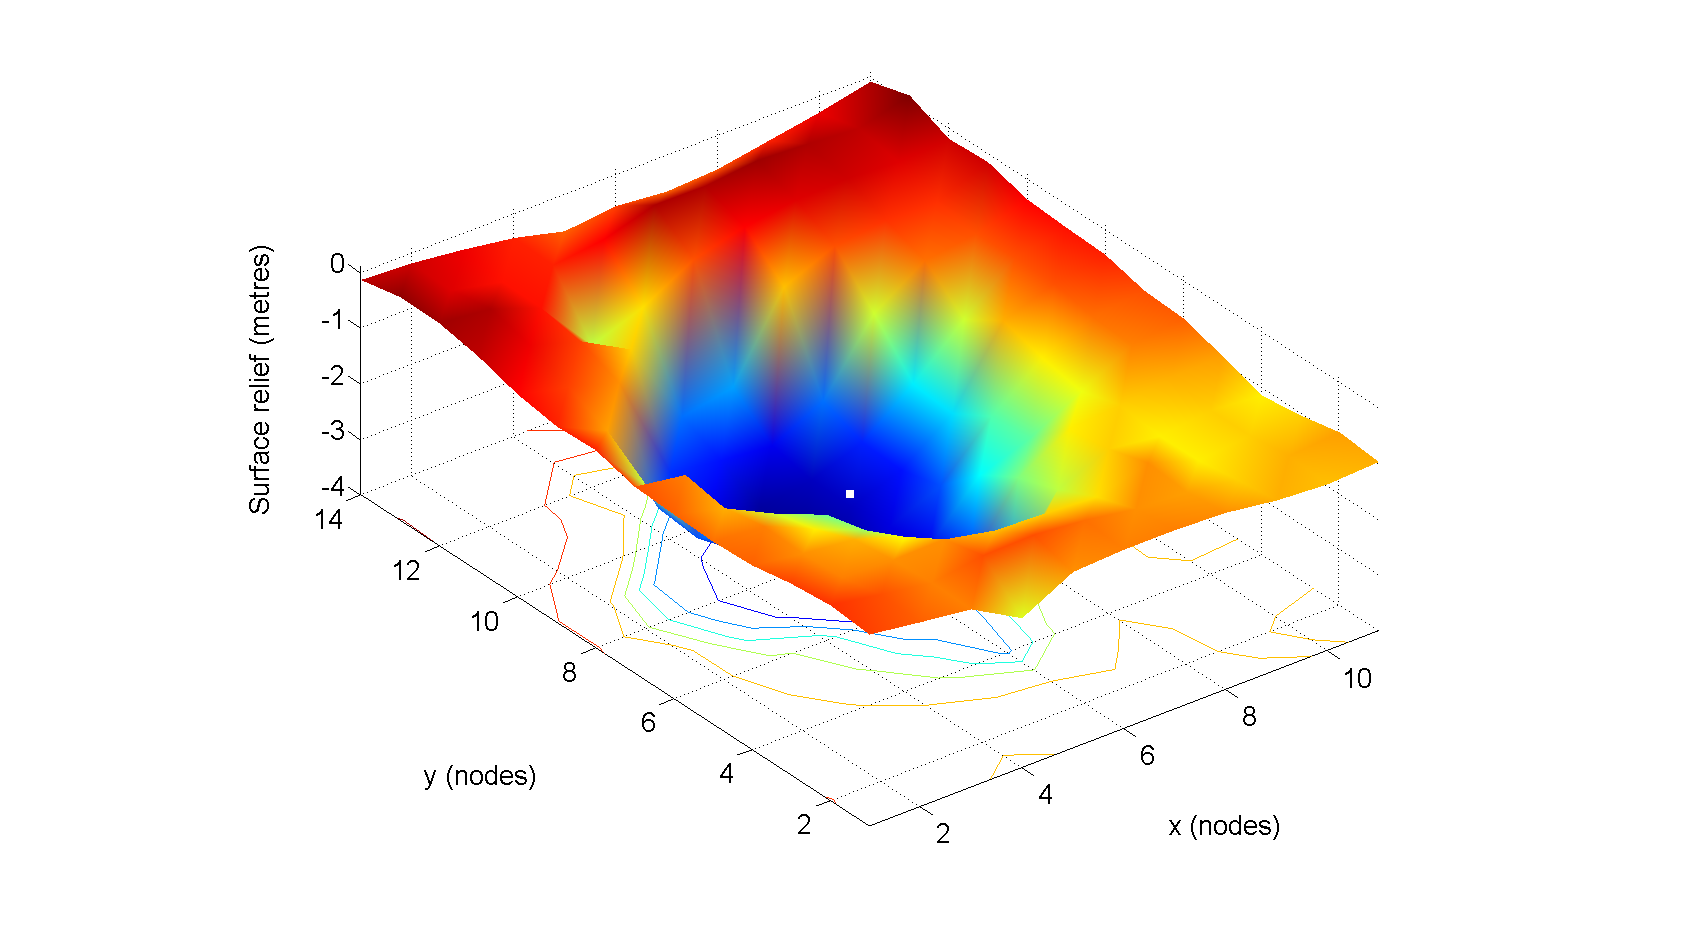
\includegraphics[scale=0.25]{fig1}
\caption{A figure sample that is not associated with the text.}
\label{fig1}
\end{figure}

\bigskip
\goodbreak

Considering the strong influence of Lomonosov's results on the
theory of invariant subspaces, it is not surprising that both
the conjecture and the techniques developed in the interesting
paper \citep{Lom91} received further attention. L.~de~Branges
used this result to obtain a characterization of the invariant
subspace problem in terms of density of certain functions. This
stimulated another characterization of the invariant subspace
problem given by Y.A.~Abramovich, C.D.~Aliprantis, and
O.~Burkinshaw ~in~\citep{AAB95}. Section~1.4 presents a more
detailed account of this work.

We take a slightly different approach. First we give a
constructive proof of the approximation theorem, inspired by
the well known Lomonosov construction used in
\citep{Lom73,RR73}. This theorem is then applied to give an
alternative proof of the main result in \citep{AAB95}. Our proof
applies to both real and complex Banach spaces, while the
original result was established for complex Banach spaces only.
The alternative proof somehow explains the role of compact
operators that appear in the characterizations of the invariant
subspace problem~\citep{AAB95}.

\medskip

\begin{table}
\caption{A sample Table}
\begin{center}
    \begin{tabular}{ | l | l | l | p{5cm} |}
    \hline
    Day & Min Temp & Max Temp & Summary \\ \hline
    Monday & 11C & 22C & A clear day with lots of sunshine.  
    However, the strong breeze will bring down the temperatures. \\ \hline
    Tuesday & 9C & 19C & Cloudy with rain, across many northern regions. Clear spells
    across most of Scotland and Northern Ireland,
    but rain reaching the far northwest. \\ \hline
    Wednesday & 10C & 21C & Rain will still linger for the morning.
    Conditions will improve by early afternoon and continue
    throughout the evening. \\
    \hline
    \end{tabular}
\end{center}
\label{tbl1}
\end{table}

One may notice that the weak*--compactness of the unit ball in
dual Banach spaces plays an important role in
\citep{AAB95,dB59,dB93,Lom91}, as well as in the applications
given in this chapter. In other words, if the Lomonosov
conjecture is true, then the compactness of the unit ball, with
respect to the weak* topology, is likely to be an important
ingredient of its proof.

\smallskip

In the last section we put this observation to the test. A
straightforward application of the approximation theorem
obtained in Section~1.3, together with the Schauder--Tychonoff
Fixed Point Theorem, yields density of non--cyclic vectors for
the dual of a convex set of compact quasinilpotent operators.
We end with the open problem of obtaining a similar result for
the original set, rather than its dual.

\bigskip

This work is more or less self--contained and the notation and
terminology used in it is (supposed to be) standard. However,
here are a few conventions that hold throughout this chapter:


\bigskip

%%% ----------------------------------------------------------------------
\goodbreak

\def\baselinestretch{1.1}

\section{Reflexive Topological Spaces and Continuous Indicator Functions}

This section introduces some topological preliminaries that
lead to a fairly general treatment of the approximation theory
in the next section, where an important role is played by the
partition of unity and the ``continuous indicator functions''
associated with a basis for the topology on a compact domain of
certain functions. The existence of continuous indicator
functions can be characterized by a purely topological property
of the underlying space, which is defined as ``reflexivity'' of
the topological space. In this section we introduce both
concepts and establish the connection between them.

\def\baselinestretch{1.66}

\begin{defn}
Let $S=(S,\tau)$ be a topological space and denote by
$C(S,\Real)$ the space of all continuous real--valued functions
on $S$. A topological space $S$ is called {\em reflexive} if
the topology $\tau$ coincides with the weakest topology
$\tau_w$ on $S$ for which all the functions in $C(S,\Real)$ are
continuous.
\end{defn}

\begin{rem}
The reflexivity of topological spaces is not to be confused
with the corresponding concept of the reflexivity of Banach
spaces. Indeed, we conclude this section by showing that every
subset of a locally convex space is reflexive.
\end{rem}

\begin{prop}
Reflexivity is a hereditary property; \, i.e. a subspace $S$ of
a reflexive topological space $X$ is reflexive with the
relative topology.
\end{prop}

\begin{proof}
Consider the restrictions of the functions in $C(X,\Real)$ to
the subset $S$, and observe that they induce the relative
topology on $S$, whenever $X$ is reflexive.
\end{proof}

\begin{defn}
Suppose $U$ is an open subset of a topological space $S$. A
continuous function $\Gamma\colon S \To \RPlus$ is called a
{\em continuous indicator function} of $U$ in $S$ if
\[ U = \set{s\in S \,\,|\,\,\, \Gamma(s) > 0}.  \]
\end{defn}

\begin{rem}
If $X$ is a metric space then every open ball
\[ U=U(x_0,r)=\set{x\in X \,\,|\,\,\, d(x,x_0) < r}, \]
admits a continuous indicator function
$\Gamma_U\colon{X}\To\RPlus$, defined by
\[ \Gamma_U(x) = \max\set{0, \, r - d(x,x_0) }. \]
Furthermore, suppose $f \in C(S,X)$. Then the open set
$V=f^{-1}(U)\subset S$ ``inherits'' an indicator function from
$U$ by setting: $\Gamma_V(s)=\Gamma_U(f(s))$.
\end{rem}

\smallskip
\goodbreak


%%% ----------------------------------------------------------------------
\goodbreak
\section{Lomonosov Functions}

The proof of the celebrated result of V.I. Lomonosov
\citep{Lom73,RR73} was based on the ingenious idea of defining a
continuous function with compact domain in a Banach space,
assuming that certain local conditions are met. In this section
we generalize this idea in the form of an approximation
theorem. Since our construction was greatly inspired by the
proof of Lomonosov's Lemma~\citep{Lom73,RR73}, we suggest the
following definition.

\begin{defn}
Let $\A \subset C(S,X)$ be a subset of the space of continuous
functions from a topological space $S$ to a locally convex
space $X$. The convex subset $\cal{L}(\A) \subset C(S,X)$,
defined by
\[ \cal{L}(\A) = \set{ \sum_{k=1}^n \alpha_k A_k \,\,|\,\,\, A_k\in\A,
   \alpha_k\in C(S,[0,1]) \text{ and } \sum_{k=1}^n\alpha_k \equiv 1;
   \,\, n < \infty}. \]

is called the {\em Lomonosov space} associated with the set
$\A$, and a function $\Lambda \in \cal{L}(\A)$ is called a {\em
Lomonosov function}.
\end{defn}

\begin{equation}
y = a + b_1x_1 + b_2x_2
\end{equation}

\medskip

Recall that the {\em uniform topology} on $C(S,X)$ is induced
by the topology on a linear space $X$. If $\cal{B}$ is a local
basis for the topology on $X$ then the sets
\[ \widehat{U}=\set{f\in C(S,X) \,\,|\,\,\, f(S)\subset U\in\cal{B}} \]
define a local basis for the uniform topology on $C(S,X)$. If
$X$ is a locally convex space then so is $C(S,X)$. In
particular, if $X$ is a Banach space then $C(S,X)$ with the
uniform topology is a Banach space, as well.

\medskip

We are now ready to give a construction of the Lomonosov
function that uniformly approximates a continuous function
within a given neighborhood.


%%% ----------------------------------------------------------------------
\goodbreak

\def\baselinestretch{1.1}

\section{Subspace Problem}

We introduce some basic concepts and notation that is
consistent with \citep{AAB95}. However, for more details and
further references on the {\em invariant subspace problem}, the
reader is advised to consult the nicely written and
comprehensible original~\citep{AAB95}.

\def\baselinestretch{1.66}
\medskip


%%% ----------------------------------------------------------------------

%\include{Ch2}
%\include{Ch3}
%\include{Ch4} 
%\include{Ch5}
%\include{Ch6} 
% ......
%\include{EvaluationAndDiscussion}
% ------------------------------------------------------------------------
% -*-TeX-*- -*-Hard-*- Smart Wrapping
% ------------------------------------------------------------------------
\def\baselinestretch{1}

\chapter{Discussion and Conclusion}

\def\baselinestretch{1.66}

%%% ----------------------------------------------------------------------

In this chapter we firstly evaluate our experimental results using statistical significance tests, then discuss the strengths and limits of our methods, and finally  draw conclusions and make some suggestions for further work. 

%%% ----------------------------------------------------------------------
\goodbreak
\section{Evaluation and Discussion}

Normally you should have a chapter before conclusion chapter, particularly for describing evaluation and discussion on your work as a whole. If you do not have such a chapter, you should have at least a Section dedicated to this, before giving conclusion and suggestion for further work.

%\bigskip

%%% ----------------------------------------------------------------------
\goodbreak
\section{Conclusions}

write your conclusions in this section.
Every point of your conclusions must have been evaluated and discussed in the previous Chapter or Section 

%%% ----------------------------------------------------------------------
\goodbreak
\section{Suggestion for Further Work}

 

% ------------------------------------------------------------------------
\setlinespacing{1.44}
%\bibliographystyle{amsplain}
\bibliographystyle{apalike}
\bibliography{xbib}

%#### Include any appendix below #####
\appendix
%% ------------------------------------------------------------------------
% -*-TeX-*- -*-Hard-*- Smart Wrapping
% ------------------------------------------------------------------------
\def\baselinestretch{1}

\chapter{On Invariant Subspaces of Essentially Self--Adjoint Operators}

\def\baselinestretch{1.66}

%%% ----------------------------------------------------------------------

An application of the main result of the previous chapter to
the algebra generated by an essentially self--adjoint operator
$A$ yields the existence of nonzero vectors $x,y\in\h$ such
that $\tau(p)=\seq{p(A)x,y}$ is a positive functional on the
space of all polynomials on the essential spectrum of $A$. This
result immediately implies the existence of real invariant
subspaces for essentially self--adjoint operators acting on a
complex Hilbert space. Elementary convex analysis techniques,
applied to the space of certain vector states, yield the
existence of invariant subspaces for essentially self--adjoint
operators acting on an infinite--dimensional real Hilbert
space.

%%% ----------------------------------------------------------------------
\goodbreak
\section{Introduction}

The existence of invariant subspaces for compact perturbations
of self--adjoint operators appears to be one of the most
difficult questions in the theory of invariant
subspaces~\cite{Lom92}. The positive results about the
existence of the invariant subspaces for the Schatten--class
perturbations of self--adjoint operators, acting on a complex
Hilbert space, date back to the late 1950's. For the facts
concerning such operators see Chapter~6 in~\cite{RR73}, where a
brief history of the problem, together with the references to
the related topics is given. The proofs of those results are
based on the concept of the separation of spectra. However,
Ljubi\v{c} and Macaev~\cite{LM65} showed that there is no
general spectral theory by constructing an example of an
operator $A$ such that $\sigma(A|\cal{M})=[0,1]$ whenever
$\cal{M}$ is a nonzero invariant subspace for $A$. This
suggests that different techniques might be needed to establish
the existence of invariant subspaces for essentially
self--adjoint operators.

\smallskip

The fact that the right--hand side of the
inequality~(\ref{e:ESSCON}) depends only on the essential norm
of the real part of the operator $A$, suggests that
Proposition~\ref{p:ESS} might have applications to the
invariant subspace problem for compact perturbations of
self--adjoint operators. In this chapter we apply
Proposition~\ref{p:ESS} in order to construct positive
functionals $\tau(p)=\seq{p(A)x,y}$ on the space of all
polynomials restricted to the essential spectrum of $A$.
Finally, in the case when the underlying Hilbert space is real,
the existence of invariant subspaces for $A$ is established
after solving an extreme problem concerning certain convex
subspaces of vector states.

\begin{defn}
Suppose $\h$ is a real or complex Hilbert space. An operator
$A\in\BH$ is called \emph{essentially self--adjoint}, if
$\pi(A)$ is a self--adjoint element in the Calkin algebra
$\BH/\KH$, where $\pi\colon\BH\To\BH/\KH$ is the quotient
mapping.
\end{defn}

\begin{rem}
Clearly, by definition of the Calkin algebra, $A$ is
essentially self--adjoint if and only if $A=S+K$, where
$S\in\BH$ is self--adjoint and $K$ is a compact operator.
Hence, saying that $A$ is essentially self--adjoint, is the
same as saying that $A$ is a compact perturbation of a
self--adjoint operator. Note, however, that this is
{\em{}false} if we replace self--adjoint operators by normal
ones.
\end{rem}

%%% ----------------------------------------------------------------------
\goodbreak
\section{On Real Invariant Subspaces}

Recently V.I.~Lomonosov~\cite{Lom92} proved that every
essentially self--adjoint operator acting on a complex Hilbert
space has a nontrivial closed \emph{real} invariant subspace.
We give an alternative proof, based on Proposition~\ref{p:ESS},
and thus introduce the idea that will be later generalized in
order to yield the existence of proper invariant subspaces for
essentially self--adjoint operators acting on a real Hilbert
space.

Recall that a \emph{real subspace} of a complex Hilbert space
$\h$ is a subset that is closed under addition and
multiplication by the \emph{real} scalars. A real subspace
$\cal{M}\subset\h$ is invariant for an operator $A\in\BH$ if
and only if $\cal{M}$ is invariant under all operators in the
\emph{real} algebra generated by $A$, i.e. the algebra of all
real polynomials in $A$.

\begin{prop}\label{p:RIS}
Suppose $\h$ is an infinite--dimensional complex Hilbert space
and let $\A$ be a convex set of commuting essentially
self--adjoint operators. Then the set of non--cyclic vectors
for $\A$ is dense in $\h$.
\end{prop}

\begin{proof}
Suppose not; then there exists a unit vector $f_0$ and a
positive number $r\in(0,1)$ such that all vectors in the set
\[  \s=\set{f\in\h\,\,|\,\,\,\norm{f_0-f}\leq\tfrac{r}{\sqrt{1-r^2}}}, \]
are cyclic for $\A$. In particular, for every vector $g\in\h$
and $\norm{g}\leq1$, there exists an operator $A\in\A$ such
that
\[ \RE\seq{A\left(f_0+\tfrac{r}{\sqrt{1-r^2}}g\right),
          -i\left(f_0-\tfrac{\sqrt{1-r^2}}{r}g\right)} > 0, \]
or equivalently,
\[ \RE\seq{ i A\left(f_0+\tfrac{r}{\sqrt{1-r^2}}g\right),
                     f_0-\tfrac{\sqrt{1-r^2}}{r}g} > 0. \]
Since $A$ is an essentially self--adjoint operator, it follows
that
\[ \essnorm{\IM{A}}=\essnorm{\RE(i{A})}=0, \]
and consequently the convex set
$i\A=\set{i{A}\,\,|\,\,\,A\in\A}$, satisfies the hypothesis of
Proposition~\ref{p:ESS}. Therefore, there exists an element
$A_0\in\A$ ($A_0\neq{z}I$), with an eigenvector $f_1\in\s$.
Since the operators in $\A$ commute, $f_1$ cannot be a cyclic
vector for $\A$, contradicting the assumption that all vectors
in $\s$ are cyclic for $\A$.
\end{proof}

\begin{cor}[V.I.\,Lomonosov, 1992]
Every essentially self--adjoint operator on an
infinite--dimensional complex Hilbert space has a nontrivial
closed real invariant subspace.
\end{cor}

\begin{proof}
The commutative algebra $\A_{\Real}$ of all real polynomials in
$A$ consists of essentially self--adjoint operators whenever
$A$ is essentially self--adjoint. By Proposition~\ref{p:RIS}
the set of non--cyclic vectors for $\A_{\Real}$ is dense in
$\h$. Since for every nonzero vector $f\in\h$ the closure of
the orbit $\A_{\Real}f=\set{T{f}\,\,|\,\,\,T\in\A_{\Real}}$ is
a real invariant subspace for $A$, it follows that $A$ has a
nontrivial closed real invariant subspace.
\end{proof}

\begin{rem}
If $A$ is a self--adjoint operator acting on a complex Hilbert
space $\h$, then for every vector $f\in\h$ and every real
polynomial $p$ we have:
\begin{equation} \label{e:I0}
  \IM\seq{p(A){f},f}=0.
\end{equation}
The condition (\ref{e:I0}) in fact characterizes self--adjoint
operators on a complex Hilbert space~\cite[p.~103]{KR83}.
Roughly speaking, Proposition~\ref{p:RIS} and its corollary
establish a similar fact for essentially self--adjoint
operators acting on a complex Hilbert space.
\end{rem}

%%% ----------------------------------------------------------------------
\goodbreak
\section{The Space of Vector States}

In the previous section we applied our machinery only to the
imaginary part of an essentially self--adjoint operator $A$. An
application to the real part yields the existence of ``vector
states'' on the space of all polynomials restricted to the
essential spectrum of $A$. Before proceeding, we make the
following conventions that hold through the rest of this
chapter:

\bigskip

As usual, let $\h$ be an infinite--dimensional real or complex
Hilbert space. The underlying field of real or complex numbers
(respectively) is denoted by $\Field$. Suppose $A\in\BH$ is a
fixed essentially self--adjoint operator without non--trivial
closed invariant subspaces and let $E$ denote its essential
spectrum. Furthermore, we may assume that $\essnorm{A}\leq1$,
and consequently, $E\subset[-1,1]$. Let $\A\subset\BH$ be an
algebra generated by $A$, i.e. $\A$ is the algebra of all
polynomials $p(A)$ with the coefficients in the underlying
field $\Field$.

\medskip

\noindent The algebra of all polynomials with the coefficients
in $\Field$, equipped with the norm
\[ \norm{p}_\infty=\max_{t\in{E}} \abs{p(t)}, \]
is denoted by $\Poly$.

\smallskip

\begin{defn}
Let $\EssD\subset\h$ be the set of all nonzero vectors $x\in\h$
for which there exists a nonzero vector $y\in\h$ satisfying the
following inequality for every polynomial $p\in\Poly$
\begin{equation} \label{e:PF1}
  \RE\seq{p(A)x,y} \leq \norm{\RE p}_\infty\seq{x,y}.
\end{equation}
\end{defn}

\medskip

\goodbreak

\begin{lem}\label{l:PF1}
The set $\EssD$ is dense in $\h$.
\end{lem}

\begin{proof}
Since the operator $A$ has no invariant subspaces the condition
of Proposition~\ref{p:ESS} is never satisfied for the algebra
$\A$. More precisely, for every unit vector $f_0\in\h$ and any
positive number $r\in(0,1)$ there exists a vector $g\perp{}f_0$
such that for every polynomial $p\in\Poly$
\[ \RE\seq{p(A)\left(f_0+\tfrac{r}{\sqrt{1-r^2}}g\right),
                  f_0-\tfrac{\sqrt{1-r^2}}{r}g} \leq
   \essnorm{\RE{}p(A)}(1 - \norm{g}^2). \]
Clearly, for every polynomial $p\in\Poly$ we have
\[ \essnorm{\RE p(A)} = \essnorm{(\RE p)(A)} = \norm{\RE p}_\infty. \]
The vectors
\[ x=f_0+\tfrac{r}{\sqrt{1-r^2}}g
   \quad \text{ and } \quad
   y=f_0-\tfrac{\sqrt{1-r^2}}{r}g \]
satisfy the inequality (\ref{e:PF1}). Letting $r\to0$, and
replacing the vector $x$ by $\lambda{x}$, where $\lambda>0$,
implies the required density of $\EssD$.
\end{proof}

\begin{lem} \label{l:PF2}
For fixed vectors $x,y\in\h$ define a linear functional
$\tau\colon\Poly\To\Field$
\[ \tau(p) = \seq{p(A)x,y}. \]
Then $\tau$ is a bounded positive functional on the space
$\Poly$ if and only if the following inequality is satisfied
for every polynomial $p\in\Poly$:
\[ \RE\seq{p(A)x,y} \leq \norm{\RE p}_\infty\seq{x,y}. \]
\end{lem}

\begin{proof}
Suppose that $\tau$ is a positive functional on $\Poly$. Then
$\RE \seq{p(A)x,y} = \seq{(\RE p)(A)x,y}$. Since $\norm{\RE
p}_\infty - \RE p$ is a positive polynomial on $E$, we have
\[ \tau(\norm{\RE p}_\infty - \RE p) =
   \seq{(\norm{\RE p}_\infty - \RE p)(A)x, y} \geq 0, \]
or equivalently,
\[ \RE\seq{p(A)x,y} \leq \norm{\RE p}_\infty\seq{x,y}. \]

Conversely, suppose $\tau$ is not a bounded positive functional
on $\Poly$. Then either there exists a real polynomial $p$ such
that $\IM\seq{p(A)x,y}\neq0$, or $\seq{p(A)x,y}<0$ for some
positive polynomial $p\in\Poly$. After replacing $p$ by $\pm i
p$ it is easy to see that $\IM\seq{p(A)x,y}\neq0$ contradicts
(\ref{e:PF1}). Similarly, for a positive polynomial $p$ we have
\[ \norm{\norm{p}_\infty-p}_\infty \leq \norm{p}_\infty. \]
Therefore $\seq{p(A)x,y}<0$ and $\seq{x,y}\geq0$ imply
\[ \seq{ \big(\norm{p}_\infty-p(A)\big)x,y} > \norm{p}_\infty\seq{x,y}
   \geq  \norm{\norm{p}_\infty-p}_\infty\seq{x,y}, \]
contradicting (\ref{e:PF1}). Finally, in the case when
$\seq{x,y}<0$ the inequality (\ref{e:PF1}) fails for the
polynomial $p\equiv-1$.
\end{proof}

\begin{defn}
The set of all bounded positive linear functionals on $\Poly$
is denoted by $\cal T$. For each vector $x\in\h$ define the set
\[ \cal{T}_x = \set{y\in\h\,\,|\,\,\,
               \tau(p) = \seq{p(A)x,y} \in \cal{T}}. \]
\end{defn}

\begin{lem} \label{l:PF3}
For every vector $x\in\h$, $\cal{T}_x$ is a closed convex
subset of $\h$.
\end{lem}

\begin{proof}
Convexity of the set $\cal T_x$ is obvious. It remains to prove
that the complement of $\cal T_x$ is an open subset of $\h$. If
$y\not\in\cal{T}_x$ then there exists a positive polynomial
$p\in\Poly$ such that $\seq{p(A)x, y} \not\geq 0$. In that case
there exists a weak neighborhood $\cal W$ of $y$ such that
$\seq{p(A)x,z}\not\geq0$ for every $z\in\cal W$. Consequently,
the complement of the set $\cal T_x$ is a (weakly) open subset
of $\h$.
\end{proof}

\begin{defn}
A positive functional $\tau\in\cal{T}$ is called a \emph{state}
if $\norm{\tau}=1$, or equivalently $\tau(1)=1$. The space of
all states on $\Poly$ is denoted by $\cal{T}'$. Similarly, for
every vector $x\in\h$ the set $\cal{T}'_x$ is defined by
\[ \cal{T}'_x = \set{y\in\h\,\,|\,\,\, \tau(p) =
   \seq{p(A)x,y} \in \cal{T}'}. \]
\end{defn}

\begin{rem}
From Lemma~\ref{l:PF1} and Lemma~\ref{l:PF2} it follows that
the set $\EssD$ of all vectors $x\in\h$ for which the set
$\cal{T}_x$ contains a nonzero vector is dense in $\h$. If $x$
and $y$ are nonzero vectors and $y\in\cal{T}_x$ then
$\seq{x,y}\geq0$. However, since a positive functional always
attains its norm on the identity function, the equality
$\seq{x,y}=0$ implies that $\tau(p)=\seq{p(A)x,y}=0$ for every
polynomial $p\in\Poly$, contradicting the fact that the
operator $A$ has no invariant subspaces. Therefore, the set
$\cal{T}'_x$ is nonempty for every vector $x$ in a dense set
$\EssD\subset\h$. In fact, for every vector $x\in\EssD$ the set
$\cal{T}'_x$ is the intersection of the cone $\cal{T}_x$ and
the hyperplane $\cal{M}_x=\set{y\in\h\,\,|\,\,\,\seq{y,x}=1}$.
Note also, that for nonzero vectors $x\in\EssD$ and
$y\in\cal{T}_x$, we have: $\seq{x,y}^{-1}y\in\cal{T}'_x$.
\end{rem}

\medskip

By Lemma~\ref{l:PF3} the set $\cal{T}'_x$ is a weakly closed
convex subset of $\h$. We show that the set $\cal{T}'_x$ has no
extreme points.

\smallskip

\begin{lem} \label{l:EXTR}
For every vector $x\in\h$ the set $\cal{T}'_x$ has no extreme
points.
\end{lem}

\begin{proof}
Suppose $y_0$ is an extreme point in $\cal{T}'_x$. By
definition of the set $\cal{T}'_x$, the functional
$\tau'(p)=\seq{p(A)x,y_0}$ is a state on $\Poly$. Hence,
\[ \omega(p)=\tau((1-t)p(t))=\seq{p(A)x, (1-A^*)y_0} \]
is a positive functional on $\Poly$. Consequently,
\[ y_1 = \seq{(1-A)x, y_0}^{-1}(1-A^*)y_0 \in \cal{T}'_x. \]
Similarly,
\[ y_2 = \seq{(1+A)x, y_0}^{-1}(1+A^*)y_0 \in \cal{T}'_x. \]
From
\[ y_0 = \frac{\seq{(1-A)x, y_0}}{2} y_1 +
         \frac{\seq{(1+A)x, y_0}}{2} y_2, \]
we conclude that $y_0=y_1=y_2$. Therefore,
$(1-A^*)y_0=\seq{(1-A)x,y}y_0$ implies that $y_0$ is an
eigenvector for $A^*$, contradicting the nonexistence of
invariant subspaces for the operator $A$.
\end{proof}

\begin{cor} \label{c:UNBOUND}
For every vector $x\in\h$ the set $\cal{T}'_x$ is either empty
or unbounded.
\end{cor}

\begin{proof}
By the Krein--Milman Theorem the set $\cal{T}'_x$ cannot be
weakly compact due to the lack of extreme points.
\end{proof}

\medskip

Although the set $\cal{T}'_x$ is unbounded for every vector
$x\in\EssD$, the following lemma shows that it contains no line
segments of infinite length. In particular, $\cal{T}'_x$ is a
\emph{proper} subset of the hyperplane
\[ \cal{M}_x=\set{y\in\h\,\,|\,\,\,\seq{y,x}=1}. \]

\medskip

\begin{lem} \label{l:FL}
Every line segment in $\cal{T}'_x$ has a finite length.
\end{lem}

\begin{proof}
Suppose the set $\cal{T}'_x$ contains a line segment of
infinite length. Then there exists a vector $y\in\cal{T}'_x$,
and a unit vector $u\perp{x}$ such that $y+\lambda
u\in\cal{T}'_x$ for every $\lambda\geq0$. For every power
$k=0,1,\ldots$, and every vector $z\in\cal{T}'_x$, we have:
$\abs{\seq{A^k x,z}}\leq1$. Applying this inequality to a
vector $y+\lambda u$ and letting $\lambda\to\infty$ implies
that $\seq{A^k x,u}=0$, contradicting the fact that $x$ is a
cyclic vector for $A$.
\end{proof}

%%% ----------------------------------------------------------------------
\goodbreak
\section{Invariant Subspaces on a Real Hilbert Space}

In this section we use vector states in order to establish the
existence of invariant subspaces for essentially self--adjoint
operators acting on an infinite--dimensional real Hilbert
space. The invariant subspace problem for essentially
self--adjoint operator will be translated into an extreme
problem and the solution will be obtained upon differentiating
certain functions at their extreme. Once again we will employ
the differentiability of the Hilbert norm. We start with the
following lemma.

\begin{lem}\label{l:DIFF}
Suppose $x$ and $y$ are any vectors in $\h$ such that
$\RE\seq{x,y}=1$. Fix a nonzero operator $T\in\BH$ and let
$a=(\norm{T}\norm{x}\norm{y})^{-1}$. Then for every vector
$z\in\h$ the function $\psi(\lambda)\colon(-a,a)\To\RPlus$,
defined by
\[ \psi(\lambda) = \norm{
   \big(\RE\seq{(1+\lambda T)y, x}\big)^{-1} (1+\lambda T)y - z}^2 \]
is differentiable on $(-a,a)$. Furthermore, if $\psi'$ denotes
the derivative of $\psi$ then
\[ \psi'(0) = 2\RE\seq{T y, y - z - (\norm{y}^2-\RE\seq{y,z}) x}. \]
\end{lem}

\begin{proof}
Since for $\lambda\in(-a,a)$ we have $\RE\seq{(1+\lambda T)y,
x}>0$, it follows that the function $\psi$ is well defined on
$(-a,a)$. In order to compute its derivative $\psi'(0)$ first
apply the polar identity to $\psi$ and then use the product and
chain rules for differentiation. A straightforward calculation
yields the required formula.
\end{proof}

\begin{defn}
For every vector $x\in\EssD$, define $P_x\colon\h\To\cal{T}'_x$
to be the projection to the set $\cal{T}'_x$, \,\,i.e. for
every $z\in\h$
\[ \norm{P_x z - z} = \inf_{y\in\cal{T}'_x} \norm{y-z}. \]
\end{defn}

\begin{rem}
Since for $x\in\EssD$ the set $\cal{T}'_x$ is nonempty, closed,
and convex it follows that the projection $P_x$ is well defined
on the whole space $\h$.
\end{rem}

\medskip

\begin{lem}\label{l:REIS}
If $x\in\EssD$ then for every vector $z\in\h$ and every power
$k=0,1,\ldots$, the following condition is satisfied:
\[ \RE\seq{A^k\big((\norm{P_x z}^2 - \RE\seq{P_x z,z})x + (I-P_x)z\big),
   P_x z} = 0.  \]
\end{lem}

\begin{proof}
Let $T=A^{*k}$, and fix a vector $y\in\cal{T}'_x$. The function
$\Phi(\lambda)\colon(-1,1)\To\h$ is defined by
\[ \Phi(\lambda) = \seq{(1+\lambda T)y, x}^{-1} (1+\lambda T)y. \]
The same argument as in the proof of Lemma~\ref{l:EXTR} shows
that $\Phi$ is well defined and $\Phi(\lambda)\in\cal{T}'_x$
for every $\lambda\in(-1,1)$.

Choose any vector $z\in\h$ and consider the function
$\psi(\lambda)\colon(-1,1)\To\RPlus$, defined by
\[ \psi(\lambda)=\norm{\Phi(\lambda) - z}^2. \]

By Lemma~\ref{l:DIFF} the function $\psi$ is differentiable,
and
\[ \psi'(0) = 2\RE\seq{T y, y - z - (\norm{y}^2-\RE\seq{y,z}) x}. \]

By definition of the projection $P_x$ the function $\psi$
attains its global minimum at the point $\lambda=0$ whenever
$y=P_x z$. Consequently, $\psi'(0)=0$ for $y=P_x z$, which
completes the proof.
\end{proof}

\medskip

A remarkable fact is that Lemma~\ref{l:REIS} holds on a real or
complex infinite--dimensional Hilbert space. It is now easy to
establish the existence of proper invariant subspaces for
essentially self--adjoint operators acting on a real Hilbert
space.

\begin{thm}\label{t:ISR}
Every essentially self--adjoint operator acting on a real
infinite--dimensional Hilbert space $\h$ has a nontrivial
closed invariant subspace.
\end{thm}

\begin{proof}
Suppose $A$ is an essentially self--adjoint operator acting on
a real infinite--dimensional Hilbert space $\h$. We may assume
that $\essnorm{A}\leq1$. If the operator $A$ has no nontrivial
invariant subspaces then we can apply Lemma~\ref{l:REIS} and
Lemma~\ref{l:FL}. We will show that this contradicts the
non--existence of invariant subspaces for $A$.

On a real Hilbert space Lemma~\ref{l:REIS} implies that for
every $k=0,1,\ldots$:
\begin{equation*}
\begin{split}
   \RE\seq{A^k\big((\norm{P_x z}^2 - \RE\seq{P_x z,z})x + (I-P_x)z\big),
   P_x z} & = \\
      \seq{A^k\big((\norm{P_x z}^2 - \RE\seq{P_x z,z})x + (I-P_x)z\big),
   P_x z} & = \, 0.
\end{split}
\end{equation*}

Since $P_x z\neq0$ it follows that
\begin{equation*}
   y_z = \big(\norm{P_x z}^2 - \RE\seq{P_x z,z}\big)x + (I-P_x)z
\end{equation*}
is a non--cyclic vector for $\A$ whenever $x\in\EssD$. The
proof is therefore completed if we show that $y_z\neq0$ for a
suitable choice of the vector $z\in\h$.

Recall that the set $\cal{T}'_x$ lies in the hyperplane
$\cal{M}_x=\set{y\in\h\,\,|\,\,\,\seq{y,x}=1}$. By definition
of the projection $P_x$, the vector $y_z=0$ for $z\in\cal{M}_x$
if and only if $z\in\cal{T}'_x$. Lemma~\ref{l:FL} implies that
$\cal{T}'_x$ is a proper subset of the hyperplane $\cal{M}_x$
and thus completes the proof.
\end{proof}

\smallskip

\begin{rem}
Theorem~\ref{t:ISR} yields the existence of invariant subspaces
for an essentially self--adjoint operator $A$ acting on a
complex Hilbert space, whenever the operator $A$ has a matrix
representation with real coefficients. Although considerable
efforts have been made to reduce the general complex case to
the real one, so far all such attempts have been unsuccessful.
\end{rem}

\bigskip
\goodbreak

\emph{We suggest that further research in this direction is
likely going to reveal additional properties of essentially
self--adjoint operators and thus contribute to our
understanding of how such operators act on the underlying
Hilbert space in terms of invariant subspaces.}

% ------------------------------------------------------------------------

%\include{AppendixB}

% =================================================================
\end{document}
% ------------------------------------------------------------------------
